
\begin{abstract}


LLM persona control divides between trait-prompt strings and model-specific activation-steering vectors; neither offers a per-response trace from output to persona contents. We introduce \textbf{Persona-CAPS}, a retrieval-based persona framework grounded in the Cognitive-Affective Personality System \cite{mischel1995caps}: a persona is a corpus of \texttt{if (situation) then (behavior)} contingencies mined from public Experience Sampling Method data, retrieved per-situation, each fired atom logged to its source observation. An audit-loop study quantifies three structural properties paragraph baselines lack: retrieval exposes corpus-level corruption that paragraph dilution masks ($P^{\!2}$-sanity passes $0/9$ on MiniMax low-Openness under identical polarity injection); atom-level repair uses $\sim 1/3$ the paragraph-baseline character footprint at comparable fix success (byte-identical on $13/13$ paired GPT-4o cross-vendor conditions); and two audit modes (universal-recall sweep, sparse-edit triage) support deployment-time governance. Across six backbones, CAPS beats Simple-Prompt on all three backbones of PersonalityBench \cite{NPTI} (mean $+0.69/10$), delivers monotonic 1-D continuous control via mixture weights $\pi$ on all 15 (vendor $\times$ Big-Five) Mini-IPIP cells, and matches the strongest paragraph baseline ($P^{\!2}$) on the non-all-low 5-D profiles (\S~\ref{sec:4.6}; backbone-level direction-match $\geq 0.93$). Cross-family judge replication ($r = +0.951$) and a two-rater human pack triangulate the headline. Code, corpus, and logs are released.

\end{abstract}

\section{Introduction}
\label{sec:1}

LLM persona interfaces today fall into two families. \textbf{Persona-as-string} (trait labels, character cards, \textit{Simple-Prompt}, and $P^{\!2}$ \cite{jiang2023p2} paragraph-prompts in the NPTI \cite{NPTI} implementation) gives strong model-agnostic control but no per-response trace from output back to specific persona contents, no atom-level edit surface, and no situation-conditional structure, even when its content derives from trait theory. \textbf{Persona-as-vector} (IRiS \cite{IRiS}, NPTI, persona vectors \cite{anthropic2025personas}) adds mechanistic grounding but trades away closed-model usability and human-readability. Both families already achieve continuous control. \textbf{The gap we address is whether the representation also supports per-response audit, atom-level edits, and corpus-level corruption sensitivity.} This gap is binding for deployments where persona behavior must be inspected, repaired, or justified after the fact --- enterprise agent governance, companion / simulation agents, safety auditing, user-controllable persona editing --- and where a trait prompt with a higher /10 score on standard psychometrics is not a sufficient interface.

We propose \textbf{Persona-CAPS}, a retrieval-based persona framework grounded in the \textit{Cognitive-Affective Personality System} (CAPS) of \citet{mischel1995caps}: a persona is a corpus $C$ of \texttt{if (situation) then (behavior)} contingencies mined from public Experience Sampling Method (ESM) data, organised into per-(dim, polarity) cells $\{C_z\}_{z=(d,p)}$. At inference time, with a single dimension $d$ under control, the model's textual response $y$ is sampled conditionally on the atom set retrieved from a $\pi_d$-weighted mixture of that dimension's two polarity cells:
\begin{multline*}
P_\theta(y \mid q, C, \pi_d) \;=\; \sum_{p} \pi_{d,p} \;\cdot\; \\
P_\theta\big(y \mid q,\ \sigma(\mathrm{TopK}_k(q, C_{(d,p)}))\big),
\end{multline*}
where $\sigma(\cdot)$ renders the retrieved atoms into a system prompt that contains \textit{no trait labels} (the corpus is the persona), and $\pi$ is a deployer-set control parameter rather than a learned distribution. Each summand is an operational sampling pipeline (\S~\ref{sec:3}, ``Locus of probability''), not a likelihood of the black-box LLM. The mixture weights $\pi_{d,p}$ are the natural continuous control surface for trait strength (deterministic top-$k$ as the $\tau \to 0$ limit of softmax retrieval; App.~\ref{app:C}). The 5-D joint mode of \S~\ref{sec:4.6} instead fixes one cell per dimension and concatenates the five retrieved sets, $\bigcup_{d \in D} \mathrm{TopK}_k(q, C_{z_d})$.

\textbf{Contributions.} (1) A \textbf{retrieval-based, model-agnostic implementation of CAPS} complementing the activation-level family (persona vectors \cite{anthropic2025personas}, NPTI \cite{NPTI}, IRiS \cite{IRiS}): atoms are natural-language \texttt{if-\allowbreak{}then} contingencies --- personas are human-readable, end-user-editable, and every response carries a contingency-level retrieval trace (\S~\ref{app:A.3}). (2) An \textbf{empirical-grounding pipeline from public ESM data} --- 166 atoms mined from \citet{beck2022esm} with no evidence of test-set leakage (\S~\ref{app:A.4}). (3) A \textbf{calibrated continuous control surface $\pi \in [0,1]^5$}: 1-D sweep monotonic on all 15 (vendor $\times$ dim) commercial cells (\S~\ref{sec:4.5}); 5-D joint composition reaches backbone-level direction-match $\geq 0.93$ at $k_\text{per dim}{=}4$ on the non-all-low profiles (\S~\ref{sec:4.6}). (4) \textbf{Apples-to-apples PersonalityBench head-to-head} across 3 backbones $\times$ 3 methods $\times$ a uniform GPT-4o judge: CAPS beats Simple-Prompt on every backbone (mean $+0.69/10$), CAPS$-$$P^{\!2}$ closes on the two commercial backbones (\S~\ref{sec:4.4}); the strongest prompt baselines reach the same surface within 3 pp on the non-all-low backbone-level aggregates. (5) An \textbf{audit-loop study} quantifying the governance interface at $\sim 1/3$ paragraph-baseline footprint (\S~\ref{sec:4.7}; the central differentiating evidence). (6) \textbf{Open codebase, corpus and run logs}, with every quantitative table and plotted result regenerable from the frozen logs. The design space is summarised in Table~\ref{tab:design-space-main}.

\textbf{A concrete instance.} In an earlier corpus build, MiniMax-M2.7 silently polarity-inverted 2 of 104 rows in the v3.4 high-extraversion JSONL (misreading \textit{``Others charge''} as \textit{``others charge at me''} rather than \textit{``others take charge''}). The fired-atom log (\S~\ref{app:A.3}) localized both atoms; a 2-row JSONL edit plus a strengthened verbaliser prompt restored the correct direction (Mini-IPIP $-0.50 \to +0.58$, $N = 3$; \S~\ref{sec:4.3}, Figure~\ref{fig:audit-case}) --- an operation structurally unavailable to persona-as-string or persona-as-vector representations. \S~\ref{sec:4.7} makes this audit-and-fix loop systematic via controlled $K$-atom polarity injection.

\section{Related Work}
\label{sec:2}

\textbf{Persona-as-string.} PersonaAgent \cite{personaagent2025} treats persona as a system prompt iteratively re-optimised at test time; DPRF \cite{dprf2025} refines a single persona description against human ground truth; PsyAgent \cite{psyagent2026} pairs a Big Five percentile prior with Multi-Scenario Contexting and SFT/LoRA; DeepPersona \cite{deeppersona2025} mines thousands of user--ChatGPT dialogues into an 8000+-node human-attribute taxonomy. All four share a common representation choice: at runtime the model sees a monolithic string with no situation-conditional retrieval and no contingency-level edit surface --- PsyAgent's Big Five prior shapes what that string says, not how it is organised. \textbf{BIG5-CHAT} \cite{big5chat2025} trains on a 100K-dialogue grounded corpus; we share the grounding commitment but operate at inference time, zero retraining cost on persona change. \textbf{Multi-PR GPA} \cite{multiprgpa2025} cites CAPS theory but operationalises it through trait-prompt engineering; we provide the retrieval-based instantiation.

\textbf{Persona-as-vector.} \citet{anthropic2025personas} extract \textit{persona vectors} (internal activations that causally control traits like ``evil'' or ``sycophancy''); the follow-up \cite{anthropic2026emotion} extracts linear emotion-concept directions for 171 emotion words in Claude Sonnet 4.5. \textbf{NPTI} \cite{NPTI} identifies neurons that discriminate opposing Big-Five poles on PersonalityBench; \textbf{DPR} \cite{DPR} extends NPTI-style persona steering with query-adaptive persona routing; \textbf{IRiS} \cite{IRiS}, closest in spirit, uses an Identify--Retrieve--Steer pipeline over \textit{situational persona neurons}. IRiS and Persona-CAPS share the CAPS-theoretic anchor but target different research questions. The activation-level family's ``atom'' is a neuron pattern measured inside an open-weight model, and its native question is mechanistic intervention. Ours is a natural-language \texttt{if-\allowbreak{}then} contingency stored in a corpus, and its native question is a deployable governance interface (closed-model usability, human-readability, end-user atom-level editability, per-response audit trail). The two operationalisations are complementary.

\textbf{Retrieval-augmented personalisation and LLM Big Five.} PersonaRAG \cite{personarag2024} retrieves over real-time \textit{user data} for relevance; PersonaAI \cite{personaai2025} retrieves over one person's logs to mimic them. We invert both the unit (an if-then contingency rather than a user fact) and the target (a trait-level disposition rather than a specific individual). \citet{serapio2023personality} validate Big-Five inventories for LLM-persona evaluation; \citet{abdulhai2025consistent} define human-validated persona-consistency metrics; ours are in \S~\ref{sec:4}.

\textbf{Where Persona-CAPS sits in the design space.} Table~\ref{tab:design-space-main} compares CAPS against the four most directly comparable families. CAPS matches $P^{\!2}$'s control strength on saturated commercial backbones (\S~\ref{sec:4.4}) and is the only design point that combines closed-model usability, atom-level editability, per-response auditability, ESM provenance, and label-free inference --- a \textit{governance interface} rather than only a controller (\S~\ref{sec:4.7}).

\begin{table*}[t]
\centering
\fitwidth{\textwidth}{%
\begin{tabular}{lcccccc}
\toprule
Method & Closed model & Human-readable & Atom-level edit & Provenance & Label-free & Control strength \\
\midrule
Trait-label prompt & \ding{51} & \ding{51} & \ding{55} & \ding{55} & \ding{55} & medium--strong \\
$P^{\!2}$ paragraph \cite{jiang2023p2} & \ding{51} & $\triangle$ \textsuperscript{a} & \ding{55} & \ding{55} & $\triangle$ \textsuperscript{a} & \textbf{strong} \\
NPTI neuron-steering \cite{NPTI} & $\triangle$ & \ding{55} & \ding{55} & \ding{55} & \ding{55} & strong \\
IRiS situated neurons \cite{IRiS} & $\triangle$ & \ding{55} & \ding{55} & \ding{55} & $\triangle$ \textsuperscript{b} & strong \\
\textbf{Persona-CAPS (this work)} & \textbf{\ding{51}} & \textbf{\ding{51}} & \textbf{\ding{51}} & \textbf{\ding{51}} & \textbf{\ding{51}} & competitive \\
\bottomrule
\end{tabular}
}
\caption{Design-space comparison on six properties. \ding{51} holds at row-level / canonical interface granularity; \ding{55} does not hold; $\triangle$ partial or restricted. Properties: closed-model (no model-internals access); human-readable (natural-language contents); atom-level edit (a single persistent row); provenance (traceable to a human-data source); label-free at the LLM interface (the deployer selects the cell, but the LLM-facing system prompt contains no trait labels); control strength (empirical Mini-IPIP / PB quality). \textsuperscript{a}$P^{\!2}$: paragraph-level (not row-level) readability; label-free for paraphrase templates only. \textsuperscript{b}IRiS: no inference-time label string but typically \emph{calibrated} against labelled persona vectors. CAPS uniquely combines all five governance properties at competitive control.}
\label{tab:design-space-main}
\end{table*}

\section{Method}
\label{sec:3}

% paper/latex/figures/figure1_framework.tex
% Persona-CAPS framework schematic. Drop into main_body via % paper/latex/figures/figure1_framework.tex
% Persona-CAPS framework schematic. Drop into main_body via % paper/latex/figures/figure1_framework.tex
% Persona-CAPS framework schematic. Drop into main_body via \input{figures/figure1_framework.tex}.
\begin{figure}[t]
\centering
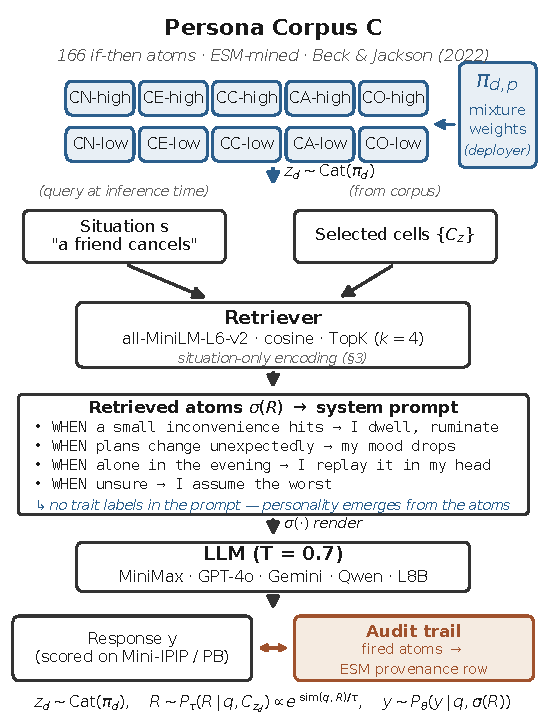
\includegraphics[width=\columnwidth]{figures/figure1_framework.pdf}
\caption{Persona-CAPS at inference. A persona is a corpus $C$ of \texttt{if-then} atoms organised into ten (dim, polarity) cells. Deployer-set mixture weights $\pi_{d,p}$ select active cells; the retriever encodes the query and each atom's situation field (\texttt{all-MiniLM-L6-v2}, cosine, top-$k{=}4$); retrieved atoms are rendered into a system prompt that contains \emph{no trait labels}; the LLM samples response $y$ at $T{=}0.7$; every fired atom is logged with provenance back to its ESM observation, yielding a per-response audit trail (\S~4.3). Conditional independencies, for a single dimension $d$ under control: $z_d \sim \mathrm{Cat}(\pi_d)$, $R \sim P_\tau(R \mid q, C_{z_d})$, $y \sim P_\theta(y \mid q, \sigma(R))$. The 5-D composition of \S~4.6 selects one $z_d$ per dimension and concatenates the five retrieved sets.}
\label{fig:framework}
\end{figure}
.
\begin{figure}[t]
\centering
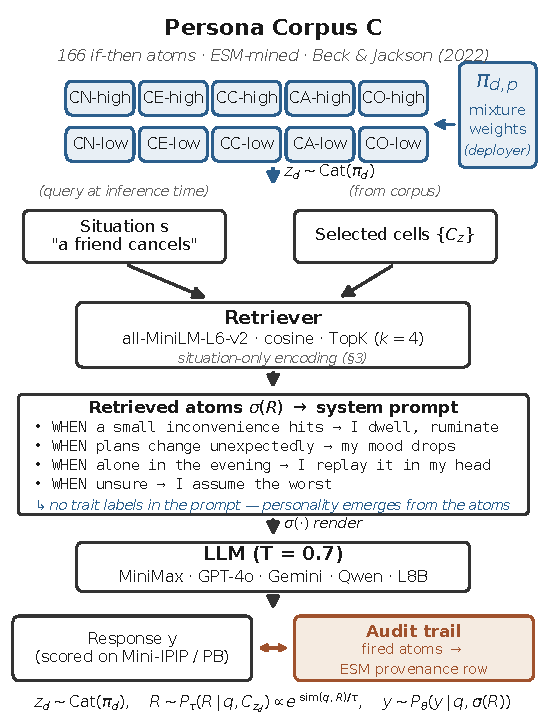
\includegraphics[width=\columnwidth]{figures/figure1_framework.pdf}
\caption{Persona-CAPS at inference. A persona is a corpus $C$ of \texttt{if-then} atoms organised into ten (dim, polarity) cells. Deployer-set mixture weights $\pi_{d,p}$ select active cells; the retriever encodes the query and each atom's situation field (\texttt{all-MiniLM-L6-v2}, cosine, top-$k{=}4$); retrieved atoms are rendered into a system prompt that contains \emph{no trait labels}; the LLM samples response $y$ at $T{=}0.7$; every fired atom is logged with provenance back to its ESM observation, yielding a per-response audit trail (\S~4.3). Conditional independencies, for a single dimension $d$ under control: $z_d \sim \mathrm{Cat}(\pi_d)$, $R \sim P_\tau(R \mid q, C_{z_d})$, $y \sim P_\theta(y \mid q, \sigma(R))$. The 5-D composition of \S~4.6 selects one $z_d$ per dimension and concatenates the five retrieved sets.}
\label{fig:framework}
\end{figure}
.
\begin{figure}[t]
\centering
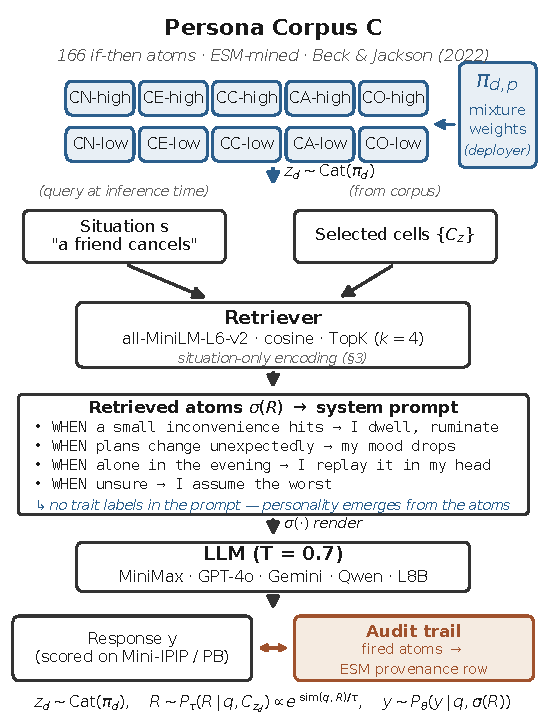
\includegraphics[width=\columnwidth]{figures/figure1_framework.pdf}
\caption{Persona-CAPS at inference. A persona is a corpus $C$ of \texttt{if-then} atoms organised into ten (dim, polarity) cells. Deployer-set mixture weights $\pi_{d,p}$ select active cells; the retriever encodes the query and each atom's situation field (\texttt{all-MiniLM-L6-v2}, cosine, top-$k{=}4$); retrieved atoms are rendered into a system prompt that contains \emph{no trait labels}; the LLM samples response $y$ at $T{=}0.7$; every fired atom is logged with provenance back to its ESM observation, yielding a per-response audit trail (\S~4.3). Conditional independencies, for a single dimension $d$ under control: $z_d \sim \mathrm{Cat}(\pi_d)$, $R \sim P_\tau(R \mid q, C_{z_d})$, $y \sim P_\theta(y \mid q, \sigma(R))$. The 5-D composition of \S~4.6 selects one $z_d$ per dimension and concatenates the five retrieved sets.}
\label{fig:framework}
\end{figure}


\textbf{Atoms, retrieval, agent.} A persona is a corpus $C = \{a_1, \ldots, a_n\}$ of \textit{if-then atoms}; each atom $a = (\text{situation},\allowbreak  \text{behavior},\allowbreak  [\text{affect}],\allowbreak  [\text{goal}],\allowbreak  [\text{dim}],\allowbreak  [\text{pol}])$ is two natural-language sentences plus optional metadata (in brackets), stored one per JSONL row --- \textit{the file is the persona}. Given a runtime situation $s$ we encode $s$ and each atom's \textit{situation field only} with \texttt{all-\allowbreak{}MiniLM-\allowbreak{}L6-\allowbreak{}v2} \cite{sbert2019} (384-dim, L2-normalised) and retrieve top-$k = 4$ atoms by cosine similarity; the agent renders these into a fixed system-prompt template (\S~\ref{app:A.1}) that contains \textbf{no trait labels}. Indexing the situation half forces a \textit{cross-target match} against the inventory item's behavioural description, foreclosing the tautological behavior-to-behavior lookup that would inflate \S~\ref{sec:4.1}. Fired atoms are logged alongside the response (\S~\ref{app:A.3}), and a localized corpus repair touches only the atoms the audit identifies --- no model retraining is involved.

\textbf{Baselines.} Two persona-as-string baselines: \textit{TraitPromptAgent} (single trait label) and \textit{PersonaDescriptionAgent} (~150-word character-card description, hand-authored without naming the trait). Two same-scaffolding ablations: \texttt{random\_\allowbreak{}demos} (chitchat atoms) and \texttt{wrong\_\allowbreak{}trait} (atoms from an orthogonal Big-Five dim at the same polarity). For \S~\ref{sec:4.4} we additionally use the \textit{Simple-Prompt} (SP) and \textit{$P^{\!2}$} paragraph-prompt baselines verbatim from \citet{NPTI}; \S~\ref{sec:4.5} adds a \textit{mixed-percentage prompt} baseline.

\textbf{Empirically grounded corpus from ESM data.} Atoms are mined from \citet{beck2022esm} (openESM \texttt{0060\_\allowbreak{}beck}, CC BY-NC 4.0) via a 6-step pipeline (\S~\ref{app:A.6}) that bins participants by trait quartiles, crosses eight DIAMONDS situation-perception items \cite{rauthmann2014diamonds} and 18 binary context flags against each behavioral item, retains $(\text{situation}, \text{behavior})$ cells with $|d_\text{high} - d_\text{low}| \geq 0.3$ (our operationalisation of \citet{mischel1995caps}'s if-then behavioral signature), and verbalises each into a first-person if-then atom via MiniMax-M2.7; every atom carries a \texttt{provenance} dict. \textbf{Released corpus}: 166 atoms across 10 (dim $\times$ polarity) cells, mean $|d| = 0.51$. \textbf{No-leakage validation} (\S~\ref{app:A.4}): trigram-Jaccard with any Mini-IPIP item $\leq 0.134$ ($0/20 \geq 0.20$); 16 / 20 items have their globally nearest atom in a \textit{non-target} cell.

\textbf{Locus of probability.} Equation (1) is an \textbf{operational mixture over prompting contexts}, not a likelihood of the black-box LLM: each summand is a concrete sampling pipeline (draw cell $z$, retrieve top-$k$, prepend, sample $y$ at $T=0.7$), with $\pi$ deployer-set. Softmax retrieval at $\tau = 1.0$ preserves $\approx$87\% of the deterministic top-$k$ spread (App.~\ref{app:C}). The four CAPS-theoretic design choices that distinguish this from generic RAG-prompting are operationalised in \S~\ref{sec:4.2} and \S~\ref{sec:4.3}.

\section{Experiments and Results}
\label{sec:4}

We address seven research questions targeting the \S~\ref{sec:1} contributions: trait fidelity (\S~\ref{sec:4.1}), content-specificity (\S~\ref{sec:4.2}), compositional editing (\S~\ref{sec:4.3}), PersonalityBench head-to-head (\S~\ref{sec:4.4}), continuous strength (\S~\ref{sec:4.5}), 5-D joint composition (\S~\ref{sec:4.6}), and audit-loop efficiency (\S~\ref{sec:4.7}). \S~\ref{sec:4.1}--\S~\ref{sec:4.6} establish standard-control parity; \S~\ref{sec:4.7} makes the governance argument. Diagnostic null and conditional-probability sweeps live in App.~\ref{app:B}--C.

\subsection{RQ1 --- Stable, measurable Big Five expression on Mini-IPIP, replicated across three vendors}
\label{sec:4.1}

\textbf{Mini-IPIP as a controlled diagnostic, not sufficient evidence.} Following the methodological cautions of \citet{serapio2023personality} and \citet{abdulhai2025consistent}, \S~\ref{sec:4.1} uses Mini-IPIP as a \textit{controlled diagnostic} of trait expression under a fixed prompt template across all conditions; we do \textit{not} treat its score as evidence that an LLM ``has'' the corresponding trait. The load-bearing behavioural evaluation is the \S~\ref{sec:4.4} head-to-head on free-response PersonalityBench against the same SP and $P^{\!2}$ baselines.

\textbf{Setup.} 20-item Mini-IPIP \cite{donnellan2006miniipip} (5-point Likert, theoretical spread range $\pm 4$) under five conditions (CAPS, \texttt{trait\_\allowbreak{}label}, \texttt{persona\_\allowbreak{}description}, \texttt{random\_\allowbreak{}demos}, \texttt{wrong\_\allowbreak{}trait}; \S~\ref{sec:3}) on three subject backends (MiniMax-M2.7-highspeed, hereafter MM; GPT-4o-2024-08-06; Gemini-2.5-Flash) at $T = 0.7$, $N = 5$ runs per cell. Bootstrap 95\% CIs (10,000 resamples) on per-run mean target spread $M(\text{high}) - M(\text{low})$; only \texttt{LLMClient} differs across backends.

\begin{table*}[t]
\centering
\fitwidth{\textwidth}{%
\begin{tabular}{lrrrrr}
\toprule
backend & \texttt{caps} & \texttt{trait\_\allowbreak{}label} & \texttt{persona\_\allowbreak{}desc} & \texttt{random\_\allowbreak{}demos} & \texttt{wrong\_\allowbreak{}trait} \\
\midrule
MiniMax-M2.7-highspeed & \textbf{+2.51} [+2.32, +2.73] & +2.69 [+2.62, +2.77] & +2.36 [+2.25, +2.51] & $-$0.01 [$-$0.06, +0.05] & $-$0.19 [$-$0.31, $-$0.07] \\
GPT-4o-2024-08-06 & \textbf{+3.74} [+3.69, +3.79] & +3.49 [+3.44, +3.55] & +3.53 [+3.50, +3.57] & $-$0.04 [$-$0.11, +0.03] & +0.08 [$-$0.03, +0.19] \\
Gemini-2.5-Flash & \textbf{+3.99} [+3.97, +4.00] & +3.77 [+3.71, +3.82] & +3.84 [+3.76, +3.92] & +0.06 [+0.01, +0.13] & $-$0.13 [$-$0.30, +0.02] \\
\bottomrule
\end{tabular}
}
\caption{Mini-IPIP target-dimension spread on three commercial backbones under CAPS retrieval vs. two prompt baselines and two scaffolding ablations. CAPS is the only condition that combines a competitive spread with a near-zero collapse on the \texttt{wrong\_trait} ablation. Bootstrap 95\% CIs from 10{,}000 resamples.}
\label{tab:rq1-ablation}
\end{table*}

\textbf{Observations.} CAPS \textit{beats} both string baselines with disjoint bootstrap CIs on GPT-4o and Gemini-Flash; on MiniMax CAPS ($+2.51$) and \texttt{trait\_\allowbreak{}label} ($+2.69$) have overlapping bootstrap CIs, so we do not resolve a difference between them at this sample size, and CAPS still beats \texttt{persona\_\allowbreak{}description} and both ablations. Cross-vendor Pearson $r$ on the full 25-cell per-(method, dim) spread grid is $\geq 0.92$ for every pair (full matrix in \S~\ref{app:A.7}), so the effect is a property of the representation, not of per-backend tuning.

\subsection{RQ2 --- Content-specificity ablations}
\label{sec:4.2}

RQ2 isolates whether the \S~\ref{sec:4.1} effect comes from CAPS's specific atom content or merely from having persona-shaped content in the system prompt. \textbf{Both ablations collapse to $\approx$ 0 on all three backends} (Tab.~\ref{tab:rq1-ablation}): \texttt{random\_\allowbreak{}demos} ranges $-0.04$ to $+0.06$ and \texttt{wrong\_\allowbreak{}trait} (the stronger control: same persona-like form, \textit{different trait content}) ranges $-0.19$ to $+0.08$, every CI excluding the smallest CAPS CI on the same backend by at least an order of magnitude --- ruling out both ``the effect is from in-context demonstrations'' and ``the effect is from any persona-shaped content occupying the system prompt.'' A cross-distribution check additionally rebuts the latent inventory-leakage worry: a \textit{circular-by-construction} IPIP-derived corpus (atoms paraphrased from IPIP-NEO-300 item phrasings, matched $N{=}3$) does not outperform Beck on Mini-IPIP (Beck $+2.33$ vs IPIP $+2.23$, MM) --- the abstract item bank does not yield stronger trait-spread than ESM-grounded situational atoms (full numbers in App.~\ref{app:B.3}).

\subsection{RQ3 --- Compositional editing: 10/10 directional moves from a worst-case opposing-pole base}
\label{sec:4.3}

\textbf{Setup.} For each (target dim, target polarity), we start from the corpus of the \textit{opposite} polarity (the hardest starting point), incrementally add 0 / 5 / 10 / 15 / 20 atoms from the target polarity, and re-administer the Mini-IPIP after each step ($N=3$ runs per step, mean reported, MiniMax-M2.7-highspeed). Beck v2 corpus throughout. All 10 conditions complete (raw payloads under \texttt{runs/\allowbreak{}rq3\_\allowbreak{}n3/\allowbreak{}}).

\textbf{10 / 10 conditions move the target in the predicted direction} (mean $|\Delta| = 1.38$ inventory points / 5); we additionally report a stricter $2\times$ off-target criterion (target $|\Delta| \geq 2\times$ max off-target $|\Delta|$) as an upper bound, which \textbf{4 / 10} conditions clear (high-N $5.08\times$, low-E $12.36\times$, low-A $6.00\times$, low-O $8.00\times$). The four strict winners are ``low''-targeted plus high $N$ --- edits travelling toward an off-default chat-model region; the six near-misses still move correctly but fight an off-target shift on RLHF-correlated traits (e.g., editing toward low-C drags neuroticism up by more than the target move itself). The same asymmetry recurs in \S~\ref{sec:4.4} and \S~\ref{sec:4.5}, triangulating the \textit{residual difficulty as a property of the chat model's prior, not of the representation}. Per-cell initial $\to$ final scores and per-cell off-target ratios in App.~\ref{app:A.8} (Table~\ref{tab:rq3-compositional}). Figure~\ref{fig:audit-case} shows this edit primitive on the \S~\ref{sec:1} corpus-build bug (fired-atom log localization, 2-row JSONL fix; Mini-IPIP $-0.50 \to +0.58$, $N=3$); \S~\ref{sec:4.7} makes the audit-and-fix loop systematic via controlled $K$-atom polarity injection.

% paper/latex/figures/figure2_case_study.tex
% §4.3 debug-and-fix audit case study. Drop into main_body via % paper/latex/figures/figure2_case_study.tex
% §4.3 debug-and-fix audit case study. Drop into main_body via % paper/latex/figures/figure2_case_study.tex
% §4.3 debug-and-fix audit case study. Drop into main_body via \input{figures/figure2_case_study.tex}.
\begin{figure}[!t]
\centering
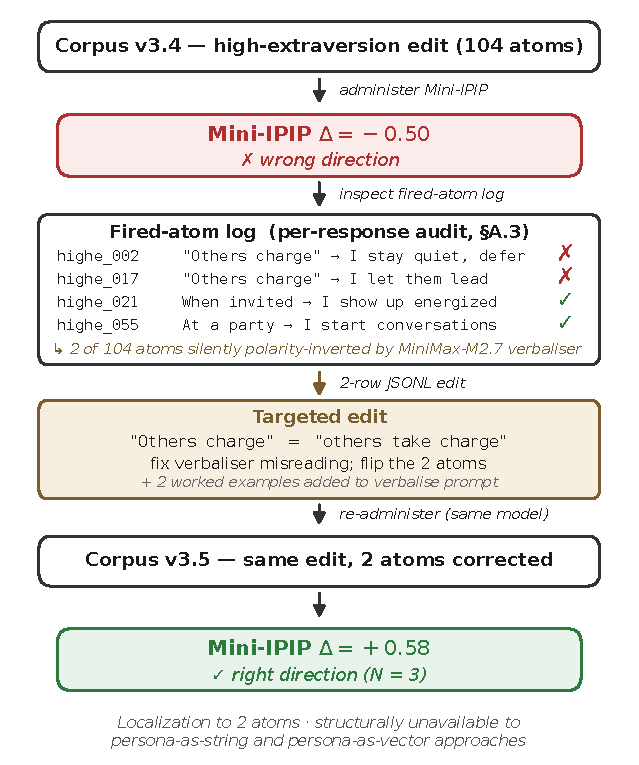
\includegraphics[width=\columnwidth]{figures/figure2_case_study.pdf}
\caption{The \S~4.3 debug-and-fix audit case at two-atom granularity. In an earlier corpus build (v3.4) the high-extraversion edit moved Mini-IPIP by \textbf{$-0.50$} (wrong direction); the fired-atom log localised the bug to \textbf{two atoms among the 104}, both reverse-keyed and both arising from the codebook phrase \texttt{"Others charge"}, which MiniMax-M2.7 misread as \texttt{"others are charging at me"} rather than \texttt{"others take charge"}, silently inverting the polarity of their first-person verbalisation. A two-row JSONL edit fixed the verbalisations; the same edit on the same model now produces \textbf{$+0.58$} ($N{=}3$). Localisation to two atoms is structurally available to a contingency-level retrieval representation and unavailable to persona-as-string and persona-as-vector approaches.}
\label{fig:audit-case}
\end{figure}
.
\begin{figure}[!t]
\centering
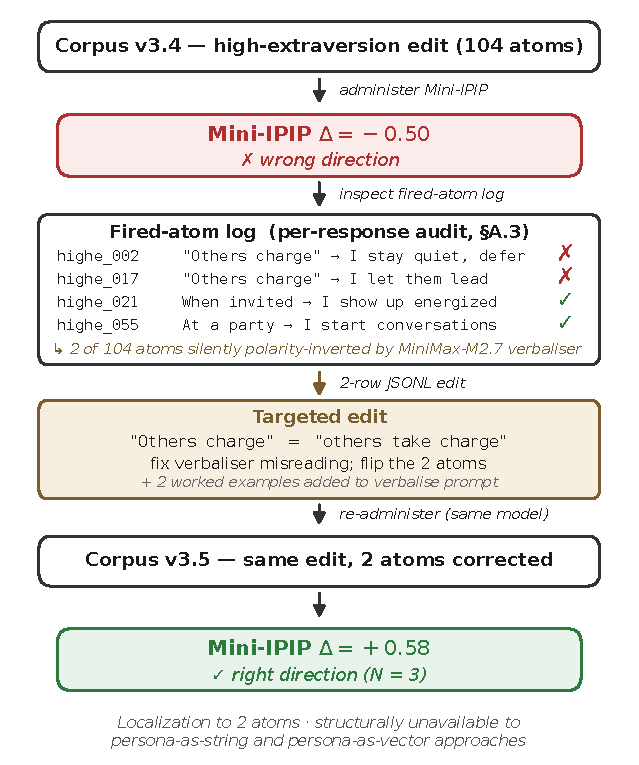
\includegraphics[width=\columnwidth]{figures/figure2_case_study.pdf}
\caption{The \S~4.3 debug-and-fix audit case at two-atom granularity. In an earlier corpus build (v3.4) the high-extraversion edit moved Mini-IPIP by \textbf{$-0.50$} (wrong direction); the fired-atom log localised the bug to \textbf{two atoms among the 104}, both reverse-keyed and both arising from the codebook phrase \texttt{"Others charge"}, which MiniMax-M2.7 misread as \texttt{"others are charging at me"} rather than \texttt{"others take charge"}, silently inverting the polarity of their first-person verbalisation. A two-row JSONL edit fixed the verbalisations; the same edit on the same model now produces \textbf{$+0.58$} ($N{=}3$). Localisation to two atoms is structurally available to a contingency-level retrieval representation and unavailable to persona-as-string and persona-as-vector approaches.}
\label{fig:audit-case}
\end{figure}
.
\begin{figure}[!t]
\centering
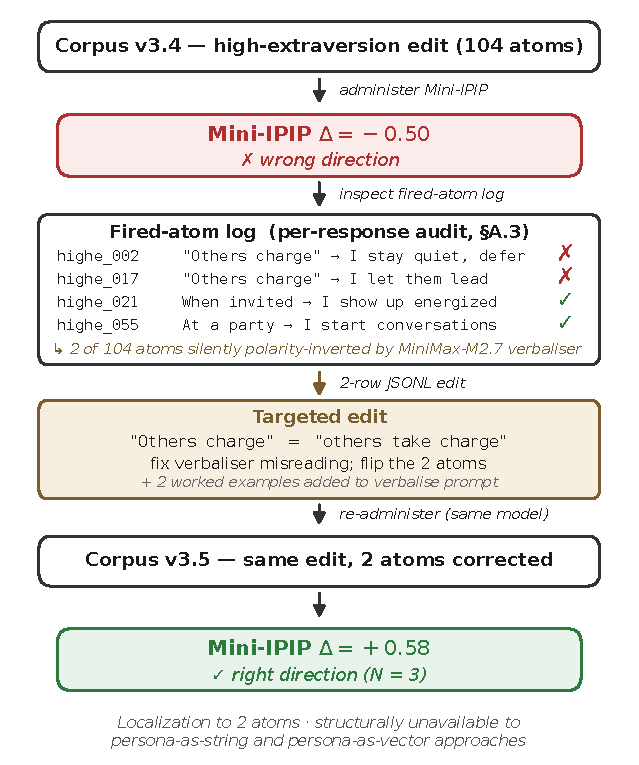
\includegraphics[width=\columnwidth]{figures/figure2_case_study.pdf}
\caption{The \S~4.3 debug-and-fix audit case at two-atom granularity. In an earlier corpus build (v3.4) the high-extraversion edit moved Mini-IPIP by \textbf{$-0.50$} (wrong direction); the fired-atom log localised the bug to \textbf{two atoms among the 104}, both reverse-keyed and both arising from the codebook phrase \texttt{"Others charge"}, which MiniMax-M2.7 misread as \texttt{"others are charging at me"} rather than \texttt{"others take charge"}, silently inverting the polarity of their first-person verbalisation. A two-row JSONL edit fixed the verbalisations; the same edit on the same model now produces \textbf{$+0.58$} ($N{=}3$). Localisation to two atoms is structurally available to a contingency-level retrieval representation and unavailable to persona-as-string and persona-as-vector approaches.}
\label{fig:audit-case}
\end{figure}


\subsection{RQ4 --- Head-to-head on the NPTI PersonalityBench protocol (3 backbones $\times$ 3 methods, uniform GPT-4o judge)}
\label{sec:4.4}

\textbf{Setup.} We replicate NPTI's PersonalityBench evaluation \cite{NPTI} (459 scenario questions, 1--5 LLM-as-judge rating, per-cell pool 89--100) and extend it to a \textbf{3$\times$3 head-to-head}: \textbf{subjects} MM, Gemini-2.5-Flash, \textbf{Llama-3-8B Q4\_K\_M} (NPTI's primary backbone, via Ollama); \textbf{methods} CAPS, \textit{Simple-Prompt} (SP) and \textit{$P^{\!2}$} \cite{jiang2023p2} paragraph-prompt (one description per call from \citet{NPTI}'s 800-description bank, 80 per cell); \textbf{judge} GPT-4o-2024-08-06 ($T=0$), held constant across all 9 cells; \textbf{budget} 50 q per (trait $\times$ polarity) cell, 4,500 judged responses total (App.~\ref{app:A.9} aggregation; raw payloads \texttt{runs/\allowbreak{}personalitybench\_\allowbreak{}*\_\allowbreak{}scored/\allowbreak{}}).

\textbf{Headline 3$\times$3 (apples-to-apples: same judge, same $N$, same templates).} All nine cells sit high on the 10-point scale and span less than a point within any backbone, so the head-to-head turns on \textit{which} traits each method moves and \textit{whether} that pattern survives a change of backbone, not on aggregate magnitude. Per-backbone, per-trait scores are in Tables~\ref{tab:pb-mm}--\ref{tab:pb-l8b} (App.~\ref{app:A.9}).

\textbf{Two findings.} \textbf{(i) CAPS exceeds SP on every backbone} ($+0.86, +0.71, +0.50$; mean $+0.69/10$), with the lift concentrated on Conscientiousness and Openness ($+0.96$ and $+1.85$ mean across the three backbones) --- the same two traits IRiS / NPTI document SP under-expressing. The CAPS$-$SP gap is therefore a generic property of substituting situated atoms for label-only prompting, not a single-backbone artefact. \textbf{(ii) The CAPS$-$$P^{\!2}$ gap is within $0.11$ pt on the two commercial backbones and closes monotonically as backbones strengthen} (L8B $-0.37$ $\to$ Gem $0.00$ $\to$ MM $+0.11$). A \texttt{-\allowbreak{}-\allowbreak{}strip-\allowbreak{}affect-\allowbreak{}metadata} template ablation on L8B recovers about a third of the residual, and the recovery is concentrated on the N/O cells \S~\ref{app:A.4.1} identifies as driving the residual, with a trade-off on $E$ rather than a unilateral gain. That cell-level agreement, rather than the size of the score change, is what identifies atom \textit{rendering} and not retrieval as the mechanism; the ablation is a diagnostic, not a deployment recommendation.

\textbf{Validation.} \citet{NPTI} publish SP $8.39$ and $P^{\!2}$ $9.43$ for this protocol, as tabulated by \citet{IRiS}; our SP-on-L8B ($8.66$) and $P^{\!2}$-on-L8B ($9.53$) sit $+0.27$ and $+0.10$ above them, a drift consistent with our 50-q-per-cell cap and Q4 quantisation (Limitations). CAPS at $9.16$ ($9.28$ with the \S~\ref{app:A.4.1} strip ablation) clears published SP but stays below the model-internals methods on the same protocol (NPTI $9.43$, IRiS $9.59$), which need weight-level access. The \textit{relative} CAPS$-$$P^{\!2}$ gap on the held-constant judge is the load-bearing comparison.

\phantomsection\label{sec:4.4.1}
\textbf{\S~4.4.1 Robustness.} Three confounds could each manufacture the CAPS$-$SP lift on their own: a judge drawn from $P^{\!2}$'s model family, CAPS's shorter answers, and an induction source shared between $P^{\!2}$ and the benchmark. App.~\ref{app:A.10} bounds all three, and none is large enough to do so --- swapping in a same-vendor judge moves the CAPS lift by under a tenth of a point, the strongest verbosity correlations sit in the baselines and not in CAPS, and $P^{\!2}$ sits closer to the benchmark's IPIP-NEO source in semantic space than the independently mined atom corpus does, with no surface-text overlap in either direction. The latter two residuals run \textit{against} CAPS, and a two-rater human pack (App.~\hyperref[app:A.10.1]{A.10.1}) agrees on the sign of the gap.

\subsection{RQ5 --- Continuous personality strength control via mixture weights $\pi_d$}
\label{sec:4.5}

Beyond polarity, do the mixture weights $\pi_{d,p}$ act as a continuous knob for the \textit{expected} trait \textit{strength}? (The within-cell $\tau_r$ moves spread only $-12.7\%$ across its range --- App.~\ref{app:C} Sweep A.)

\textbf{Setup.} Per dim $d$, activate \texttt{high\_\allowbreak{}d} / \texttt{low\_\allowbreak{}d} with weights $(w, 1-w)$, $w \in \{0, 0.25, 0.5, 0.75, 1\}$; \texttt{JointCapsAgent} draws one cell per query, \texttt{top\_\allowbreak{}k\_\allowbreak{}per\_\allowbreak{}dim = 4}. Three commercial backends (Gem, GPT-4o, MM) at $T = 0.7$, $N = 3$ runs per $w$ --- 225 administrations. We use $k = 4$ throughout as a representative control--auditability working point rather than a tuned optimum: an endpoint sweep over $k \in \{2, 4, 8\}$ (App.~\hyperref[app:A.9.9]{A.9.9}) leaves the achievable range nearly flat across a fourfold change in budget, so a larger $k$ buys almost no additional control while adding a row to every audit trail.

\textbf{Result --- monotonic control on every dimension on every vendor.} All 15 (vendor $\times$ dim) cells are \textbf{strictly monotonic in $w$} with per-cell Spearman $\rho = +1.000$, traversing $\geq 2.25$ inventory points end-to-end (joint random-ordering null $\approx 6.5 \times 10^{-32}$). Across vendors the \textit{shape} of the curve transfers almost exactly while its \textit{height} does not: every pairwise cross-vendor correlation among the three stays above $+0.97$ --- and above $+0.85$ across all five backbones once the open-weight replications are folded in (App.~\ref{app:A.7}) --- yet the mean spreads differ by more than a full inventory point between the widest and narrowest backbone. What transfers is the ordering of $\pi_d$ settings, not a fixed trait level per setting; the absolute range a backbone can reach is a property of its instruction-tuned prior. Full grids in App.~\hyperref[app:A.9.5]{A.9.5} (Table~\ref{tab:pi-grid-commercial}); open-weight replications in App.~\hyperref[app:A.9.6]{A.9.6}--7.

\textbf{What $\pi_d$ controls.} For the dimension being swept, each query samples \textit{one} polarity cell according to $\pi_d$, so the monotonicity above is the \textbf{expected trait level over repeated generations}, not interpolation within a single response. This aggregate reading is the one CAPS asks for: the theory locates personality in contingencies stable \textit{across occasions}, not in a fixed intensity realised within every act. An exploratory three-arm pilot asks whether $\pi_d$ could instead be realised \textit{within} a single prompt: retrieving both polarity cells into one prompt does narrow the response distribution (extreme-rating share $64\% \to 28\%$, and to $11\%$ once a target-free integration instruction is added), but the mean curves lose strict monotonicity and that instruction also compresses the endpoints, so the deployed knob remains the frequency axis (App.~\hyperref[app:A.9.10]{A.9.10}).

\textbf{A mixed-percentage prompt reaches the same 1-D control surface.} Asking a model directly for \textit{``X\% high pole and (100$-$X)\% low pole''} is monotonic on 14 of 15 cells and, cell by cell (Table~\ref{tab:caps-vs-promptbase}, App.~\hyperref[app:A.9.11]{A.9.11}), matches CAPS on end-to-end range and on off-target leakage while being marginally the better calibrated of the two. On the strength axis taken by itself, CAPS is therefore not the wider or the cleaner knob. What the percentage prompt cannot do is report which retrieved unit produced a given response, or let a deployer edit that unit and re-verify --- the properties \S~\ref{sec:4.7} measures. The control surface itself replicates on open-weight backbones and on a distilled reasoning subject (Qwen3.5-9B, Llama-3-8B, DeepSeek-R1-Distill-Qwen-14B; App.~\hyperref[app:A.9.6]{A.9.6}--8).

\subsection{RQ6 --- Joint 5-D Big-Five composition: $\pi$ as a multi-trait control surface}
\label{sec:4.6}

\textbf{Setup.} \texttt{JointCapsAgent} retrieves $k_\text{per dim}$ atoms from each of the five cells the profile requests (one endpoint polarity per dimension, $\pi_d \in \{0,1\}$), concatenated into one prompt. We evaluate \textbf{7 Big-Five profiles} --- HHHHH, its 5 single-flips (one trait reversed against an otherwise prosocial prior), and LLLLL (anti-prior stress) --- at $N{=}3$ runs and $k{\in}\{3, 4\}$, against a 5-D $P^{\!2}$ baseline stacked from \citet{NPTI} single-trait paragraphs (construction in App.~\ref{app:C.4}).

\textbf{How to read the table.} Direction-match asks only whether each of the five dimensions moved the way it was asked to --- the criterion a deployer can check without a calibrated scale. It is deliberately coarse: a dimension counts as matched once it clears the scale midpoint by $0.25$ inventory points in the prescribed polarity, however far short of the pole it stops. The finer measures in App.~\ref{app:C.4} (intensity, per-flip specificity, swing, cross-dimension drift) do not reverse the head-to-head, though $P^{\!2}$ does hold a small intensity-axis lead on both backbones, which we attribute to its explicit Big-Five vocabulary matching the Mini-IPIP item language rather than to better composition.

\begin{table*}[t]
\centering
\fitwidth{\textwidth}{%
\begin{tabular}{lrr}
\toprule
method & MM (all 7 / excl.\ LLLLL / LLLLL) & Gem (all 7 / excl.\ LLLLL / LLLLL) \\
\midrule
CAPS ($k_\text{per dim}{=}4$) & \textbf{0.91} / \textbf{0.93} / 0.73 & \textbf{0.97} / \textbf{1.00} / 0.80 \\
$P^{\!2}$ (NPTI stacked, App. \ref{app:C.4}) & 0.95 / 0.96 / \textbf{0.93} & 0.99 / 0.99 / \textbf{1.00} \\
\bottomrule
\end{tabular}
}
\caption{Joint 5-D Big-Five composition head-to-head on two commercial backbones (MM, Gem) at $k_\text{per dim}{=}4$. Direction-match rate over 7 profiles $\times$ $N{=}3$ runs; \texttt{excl. LLLLL} removes the anti-prior all-low profile; \texttt{LLLLL} is the anti-prior cell only. Full grid (k=3 and k=4, per-profile, intensity, specificity) in Table~\ref{tab:p2-joint-5d-headtohead} (App. \ref{app:C.4}).}
\label{tab:rq6-joint-headtohead}
\end{table*}

\textbf{On the 12 non-all-low profile--backbone cells the methods reach the same direction-match} (HHHHH + 5 single-flips $\times$ 2 backbones): 2 CAPS wins, 7 ties, 3 $P^{\!2}$ wins; overall $+1$ pp on Gemini and $-3$ pp on MM. The remaining 2 cells are LLLLL --- adversarial against the chat model's RLHF prior on every dim --- where explicit label-override prompts are structurally suited: a complementary regime, not a unified loss ($-20$ pp on both backbones; Tab.~\ref{tab:rq6-joint-headtohead}).

\subsection{RQ7 --- Audit-loop efficiency: bug injection, localization, and atom-level repair}
\label{sec:4.7}

\textbf{Motivation and experimental question.} \S~\ref{sec:4.1}--4.6 measure \textit{what} each persona method produces; \S~\ref{sec:4.7} measures \textbf{the governance interface}: what happens when the persona representation contains a contradiction, and what each method can do about it. We inject $K$ polarity-inverted atoms into the persona corpus and ask, of each representation: can it detect the corruption (sanity gate), localize the bad atoms, and repair them without collateral damage to other traits? Two CAPS audit workflows and three $P^{\!2}$ baselines are compared on localization precision / recall, post-fix restoration of the clean Mini-IPIP profile, edit footprint, and off-target preservation. Subject backbone MiniMax-M2.7-highspeed ($T = 0.7$), 3 seeds per (cell, $K$); driver and aggregation scripts in \texttt{scripts/\allowbreak{}audit\_\allowbreak{}loop/\allowbreak{}} (\texttt{aggregate.py}); raw payloads under \texttt{runs/\allowbreak{}audit\_\allowbreak{}loop/\allowbreak{}}. Mini-IPIP shifts here are a representation-shift proxy (per-cell reproducible), not a trait measurement (cf. \S~\ref{sec:4.1}).

\textbf{Pollution protocol (targeted strategy).} \textbf{For retrieval-based audit we deliberately construct the worst case:} for each (dim, polarity) cell we draw $K \in \{5, 10, 15\}$ atoms from the target cell and rewrite each \texttt{behavior} field via GPT-4o ($T=0$, strict-JSON, $\geq 1$ retry, hard-reject pure-negation rewrites) into the opposite polarity --- situation, affect, and visible metadata (\texttt{polarity}, \texttt{target\_\allowbreak{}dimension}) preserved verbatim, so the metadata still claims the atom is on-polarity. A condition is sanity-passing iff the polluted-vs-clean Mini-IPIP shift on the target dim has $|\Delta\bar{s}| \geq 1.0$ point \textit{and} at least two of the four target-dim items cross the scale midpoint (\textit{direction-match rate} $\leq 0.7$).

\textbf{Trait-asymmetric editability --- and its diagnostic value.} Mean $|\Delta\bar{s}|$ across the 9 (K, seed) conditions per cell: high-E $2.53$, low-O $2.89$, high-N $0.92$, low-A $0.83$, low-C $0.47$ (Tab.~\ref{tab:rq7-mm-sanity}). MiniMax's conscientiousness prior dominates even when 15 / 31 atoms are inverted, so the audit-loop runs on the four cells that \textit{can} be polluted (E, A, N, O). This asymmetry is itself a finding: corpus-pollution sensitivity doubles as a probe for RLHF-locked dimensions --- that low-C resists $K=15$ injection tells a deployer MM has \textit{overdetermined} conscientiousness. C-cell scope in Limitations.

\textbf{Five audit workflows, identical subject + query stream.} \textbf{CAPS-A} (incident-driven, per-response): for each Mini-IPIP item where polluted disagrees with clean in direction, flag the atom in the agent's fired-atom log whose situation most closely matches the item --- sparse by construction. \textbf{CAPS-B} (scheduled, corpus-metadata sweep): GPT-4o re-classifies every atom's behavior into $(\text{dim}, \text{polarity})$ and flags any atom whose classification disagrees with its stored \texttt{polarity} --- one-shot batch over the corpus. \textbf{$P^{\!2}$-Oracle} (upper bound): the auditor is handed the $K$ ground-truth flipped sentences in the matching $P^{\!2}$ paragraph and edits exactly those. \textbf{$P^{\!2}$-Blind}: entire D-paragraph regenerated from the trait-target prompt; no per-atom editable unit. \textbf{$P^{\!2}$-Detect}: same inventory-disagreement signal as CAPS-A, plus GPT-4o is asked which sentences are most likely responsible --- the closest $P^{\!2}$ counterpart to CAPS-A.

\textbf{$P^{\!2}$ leaves sanity-gate failures on 2 of 4 cells --- a representation-level finding. Over individual $(K, \text{seed})$ conditions $P^{\!2}$-sanity passes $0/9$ on MiniMax low-openness across $K \in \{5, 10, 15\}$ and $1/3$ on high-neuroticism at $K = 15$; only low-openness has no passing condition at all.} When the same $K$ inverted behaviors are stitched into the surrounding $\sim 320$-word $P^{\!2}$ paragraph, the unchanged trait declaration dilutes them and the resulting persona is indistinguishable from clean $P^{\!2}$ on the target dim ($|\Delta\bar{s}| < 1.0$): \textbf{retrieval surfaces corpus pollution that paragraph dilution masks}. $P^{\!2}$ metrics below are therefore reported on the matching sanity-pass subset; CAPS metrics use the full sanity-passing CAPS set.

\begin{table*}[t]
\centering
\fitwidth{\textwidth}{%
\begin{tabular}{llllll}
\toprule
cell (n) & CAPS-A P / R, fix, edits & CAPS-B P / R, fix, edits & $P^{\!2}$-Oracle P / R, fix, edits & $P^{\!2}$-Blind fix, edits & $P^{\!2}$-Detect P / R, fix, edits \\
\midrule
high-E (6) & \textbf{1.00 / 0.33}, \textbf{5 / 6}, \textbf{4} & 0.92 / 1.00, 6 / 6, 12.5 & 1.00 / 1.00, 6 / 6, 12.5 & 6 / 6, full $\sim 320$ w & 1.00 / 1.00, 4 / 6, 12.5 \\
high-N (3) & 1.00 / 0.40, 1 / 3, 6 & 1.00 / 1.00, 2 / 3, 15 & 1.00 / 1.00, 1 / 1, 15 & 1 / 1, full & 1.00 / 1.00, 1 / 1, 15 \\
low-A (2) & 0.42 / 0.15, 0 / 2, 2 & 0.92 / 1.00, \textbf{1 / 2}, 12.5 & 1.00 / 1.00, 0 / 2, 12.5 & 0 / 2, full & 1.00 / 1.00, 0 / 2, 12.5 \\
low-O (9) & 0.80 / 0.44, \textbf{6 / 9}, 4 & 0.68 / 1.00, 4 / 9, 10 & --- & --- & --- \\
\bottomrule
\end{tabular}
}
\caption{Localization, fix success, edit footprint, and off-target preservation over the four CAPS-sanity-passing cells. Means over seeds and $K$; n per cell. $P^{\!2}$-sanity pass rates: high-E 6/6, low-A 2/2, high-N 1/3, low-O 0/9 (\S~\ref{sec:4.7}); em-dash = workflow unavailable (low-O $P^{\!2}$-sanity fails). Low-A: 2 of the 9 MM (K, seed) conditions pass the sanity gate (K=10 and K=15, both seed 3; Limitations); reported on those 2. Bold = CAPS-A's sparse-edit signature: 4-atom edits, $0.32\times$ the $P^{\!2}$-Oracle footprint at comparable fix-success on high-E.}
\label{tab:rq7-audit}
\end{table*}

\textbf{Three localization patterns.} (i) \textbf{Locator B achieves $R = 1.00$ across all four cells}, with precision cell-dependent ($0.68$--$1.00$). On low-openness $P$ rises monotonically with $K$ ($0.45$ / $0.71$ / $0.88$ at $K = 5$ / $10$ / $15$), consistent with a roughly fixed false-positive count diluted by rising true positives. (ii) \textbf{Locator A is a sparse high-precision triage tool on extraversion and neuroticism} ($P = 1.00$, $R = 0.33$--$0.40$, 4--6 atoms flagged out of $K = 10$--$15$) but \textbf{degrades on low-agreeableness} ($P = 0.42$, $R = 0.15$; downstream CAPS-A fix $0/2$ on this cell): IPIP-A items semantically overlap multiple Big-Five dimensions and the fired-atom signal becomes diffuse. Locator A is cell-dependent --- on low-openness it reaches $P = 0.80$. (iii) \textbf{$P^{\!2}$-Oracle / $P^{\!2}$-Detect score $P{=}R{=}1.00$ on the three cells that have at least one $P^{\!2}$-sanity-passing condition}, but only because Oracle gets ground truth and Detect labels sentences on a 26\nobreakdash--39-atom corpus with the cell label visible --- structurally easier than CAPS's locator task.

\textbf{Two repair patterns the localization table hides.} (i) \textbf{On low-agreeableness, CAPS-B (fix 1 / 2) is the only workflow that recovers the clean persona}; $P^{\!2}$-Oracle, $P^{\!2}$-Blind, and $P^{\!2}$-Detect each achieve $0 / 2$ fixes despite Oracle being handed ground-truth atom IDs. The bottleneck is not localization: $P^{\!2}$ paragraph rewrites cannot carry the ESM-style first-person contingency the CAPS persona uses, even when the editor knows exactly what to change. (ii) \textbf{On low-openness CAPS-A (6 / 9) outperforms CAPS-B (4 / 9)} despite Locator B's perfect recall --- fix quality is bottlenecked by off-target spillover from editing 10--15 atoms at once, not by missing the ground-truth set.

\textbf{Off-target preservation: CAPS-A best, $P^{\!2}$-Detect and $P^{\!2}$-Blind worst} (mean $|\Delta\bar{s}|$ on four non-target dims). On the three cells where every workflow ran (high-E, high-N, low-A): CAPS-A $0.31$, CAPS-B $0.36$, $P^{\!2}$-Oracle $0.34$, $P^{\!2}$-Detect $0.44$, $P^{\!2}$-Blind $0.43$ (Tab.~\ref{tab:rq7-mm-offtarget}); $P^{\!2}$-Blind drifts $\sim 40\%$ more than CAPS --- the quantitative cost of paragraph-as-smallest-editable-unit. Including low-O CAPS-A grand mean $0.32$.

\textbf{Cross-vendor subject replication.} Across $13/13$ paired sanity-passing seeds the GPT-4o subject's CAPS-A flag set restores atoms with byte-identical per-seed character counts to the MiniMax subject (Tab.~\ref{tab:rq7-xvendor-byteid}) --- the edit unit is a property of the representation, not the subject. Full GPT-4o grid (off-target, $P^{\!2}$-Detect structural footprint, $P^{\!2}$-sanity regime-dependence): App.~\ref{app:A.11}~(i)--(iv).

\textbf{What the repair loop does and does not guarantee.} The workflow is \textit{localize--intervene--verify} at atom granularity: the audit marks candidate atoms, the intervention edits the \texttt{behavior} field of exactly those, and re-administering Mini-IPIP checks whether the clean profile is restored. Crucially, \textbf{there is no optimality guarantee before that verification step} --- a flagged edit is a hypothesis, and the fix-success columns above are the rate at which it survives checking. We claim an atom-granular localize--intervene--verify workflow, not root-cause analysis and not automated repair. Generating candidate fixes with verification in the loop --- propose, re-administer, revise until the profile is restored --- is the natural next step.

\textbf{Summary.} Three conclusions follow; exact per-cell values in Tab.~\ref{tab:rq7-audit}, Tab.~\ref{tab:rq7-xvendor-byteid} and App.~\ref{app:A.11}. First, \textbf{the representation decides whether corruption is visible at all}: a polluted paragraph still reads as Mini-IPIP-clean, while the same corruption is detectable once the persona is retrieved atom by atom. Second, \textbf{it decides how much must be rewritten to repair it}: CAPS-A restores the clean profile by editing a handful of flagged atoms where the paragraph baselines regenerate a whole one, with the least off-target drift of any workflow tested --- a contrast that survives a change of subject backbone, where CAPS-A's flag sets reproduce byte-for-byte. Third, \textbf{the choice of audit mode is operational, not a quality ranking}: Locator B's exhaustive recall fits scheduled sweeps, Locator A's sparse precision fits incident-driven triage, and neither dominates. Scope limits in Limitations.

\section{Discussion}
\label{sec:5}

Persona-CAPS reframes the persona representation from a control knob into an inspectable, editable, repairable artefact. \S~\ref{sec:4.5}--4.6 show that retrieval reaches the strongest paragraph baselines everywhere except the all-low stress profile; \S~\ref{sec:4.7} shows the same retrieval surfaces, locates, and repairs corpus-level pollution at $\sim 1/3$ paragraph-baseline footprint. The combination --- controllable and auditable through the same representation --- is what the title claims and what neither persona-as-string nor persona-as-vector currently delivers in a single deployable interface; $P^{\!2}$ has a clear edge on the weaker L8B backbone (\S~\ref{sec:4.4}) and on the adversarial all-low (LLLLL) profile; over the non-all-low profiles the backbone-level direction-match aggregates differ by at most 3 pp (\S~\ref{sec:4.6}).

\textbf{Paragraph representations can mask corpus corruption, and offer no sub-paragraph repair unit.} $K{=}15$ atoms inverted in a $\sim 320$-word $P^{\!2}$ paragraph leave the persona Mini-IPIP-clean --- corruption invisible at the representation level (\S~\ref{sec:4.7} $P^{\!2}$-sanity passes $0/9$ on MM low-O); retrieval surfaces it.

\textbf{Beyond persona control.} Nothing in the localize--intervene--verify loop is specific to personality: it requires only that the conditioning signal be assembled from \textit{human-readable retrieval units}. We therefore expect it to extend to other controlled-generation tasks built that way, such as style and register specifications or safety policies decomposed into retrievable rules. Persona control is the only setting we evaluate here.

